\chapter{项目内容及优化实现}\label{sec:algorithm}

本章介绍了项目在准备阶段和项目各部分优化细节。项目的准备阶段包括数据库的设计与实施、系统代码的编写以及短视频压缩编码的初步实现。优化细节包括数据库性能瓶颈分析与消除、数据库语句优化以及视频压制优化。

\section{数据库的设计}
 
\subsection{需求分析}
设计数据库首先要进行需求分析。本系统需要数据库来管理与储存用户信息、视频信息、视频的评论信息用户以及用户与视频的各种关系。用户信息包含用户的系统内唯一编号、用户名、密码、注册时间、用户头像以及用户各项统计信息等内容。视频信息包括视频名称、视频文件存放位置、视频作者、视频相关统计信息等内容。评论信息包含评论人、评论内容、评论种类、评论视频等内容。用户与视频关系包含关系类型、用户编号与视频编号等内容。

为了需求分析的简便,我们先将用户与视频所有的信息放入一张表中,其 E-R 图如图 \ref{fig:ER1} 所示。随后我们要进行关系的规范化。

\begin{figure}[!ht]
    \centering
    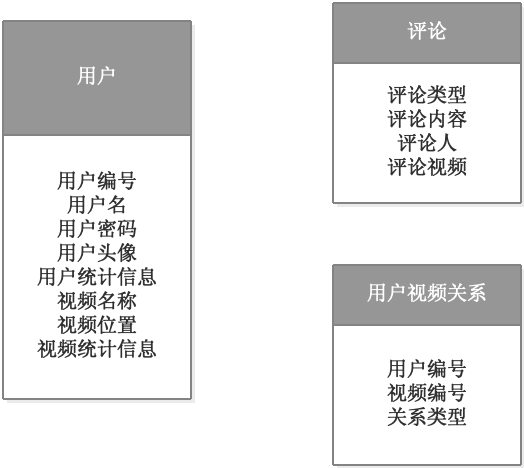
\includegraphics[width=0.5\textwidth]{dbs1.png}
    \caption{需求分析数据库 E-R 图}
    \label{fig:ER1}
\end{figure}


\subsection{关系规范化}

经过初步地需求分析后,我们得到了一个初步地数据库模型,但这个模型仅仅遵循了关系数据库理论的第一范式,即所有的属性均为原子属性。仅遵循第一范式的模型有插入异常、删除异常以及修改复杂等缺点。以此模型中的用户表为例。当一个用户没有任何视频时无法将该用户插入,导致更新异常。当一个用户信息需变更时需改变所有包含用户信息的元组,导致修改复杂。当用户删除所有视频时会导致用户信息被一同删除,导致删除异常。

为了解决这些问题,我们需要使数据库符合第二范式,即关系遵循第一范式,且关系中所有的非主属性都完全函数依赖于任何候选码。为了使关系遵循第二范式,我们要对其进行规范化,即将一个大的关系拆分为两个或多个小的关系。我们将用户表拆分为用户信息表和视频信息表,两个表的函数依赖关系在拆分后由外健保留,关系拆分后 E-R 图 (省略实体的属性) 如图 \ref{fig:ER2} 所示 。

\begin{figure}[!ht]
    \centering
    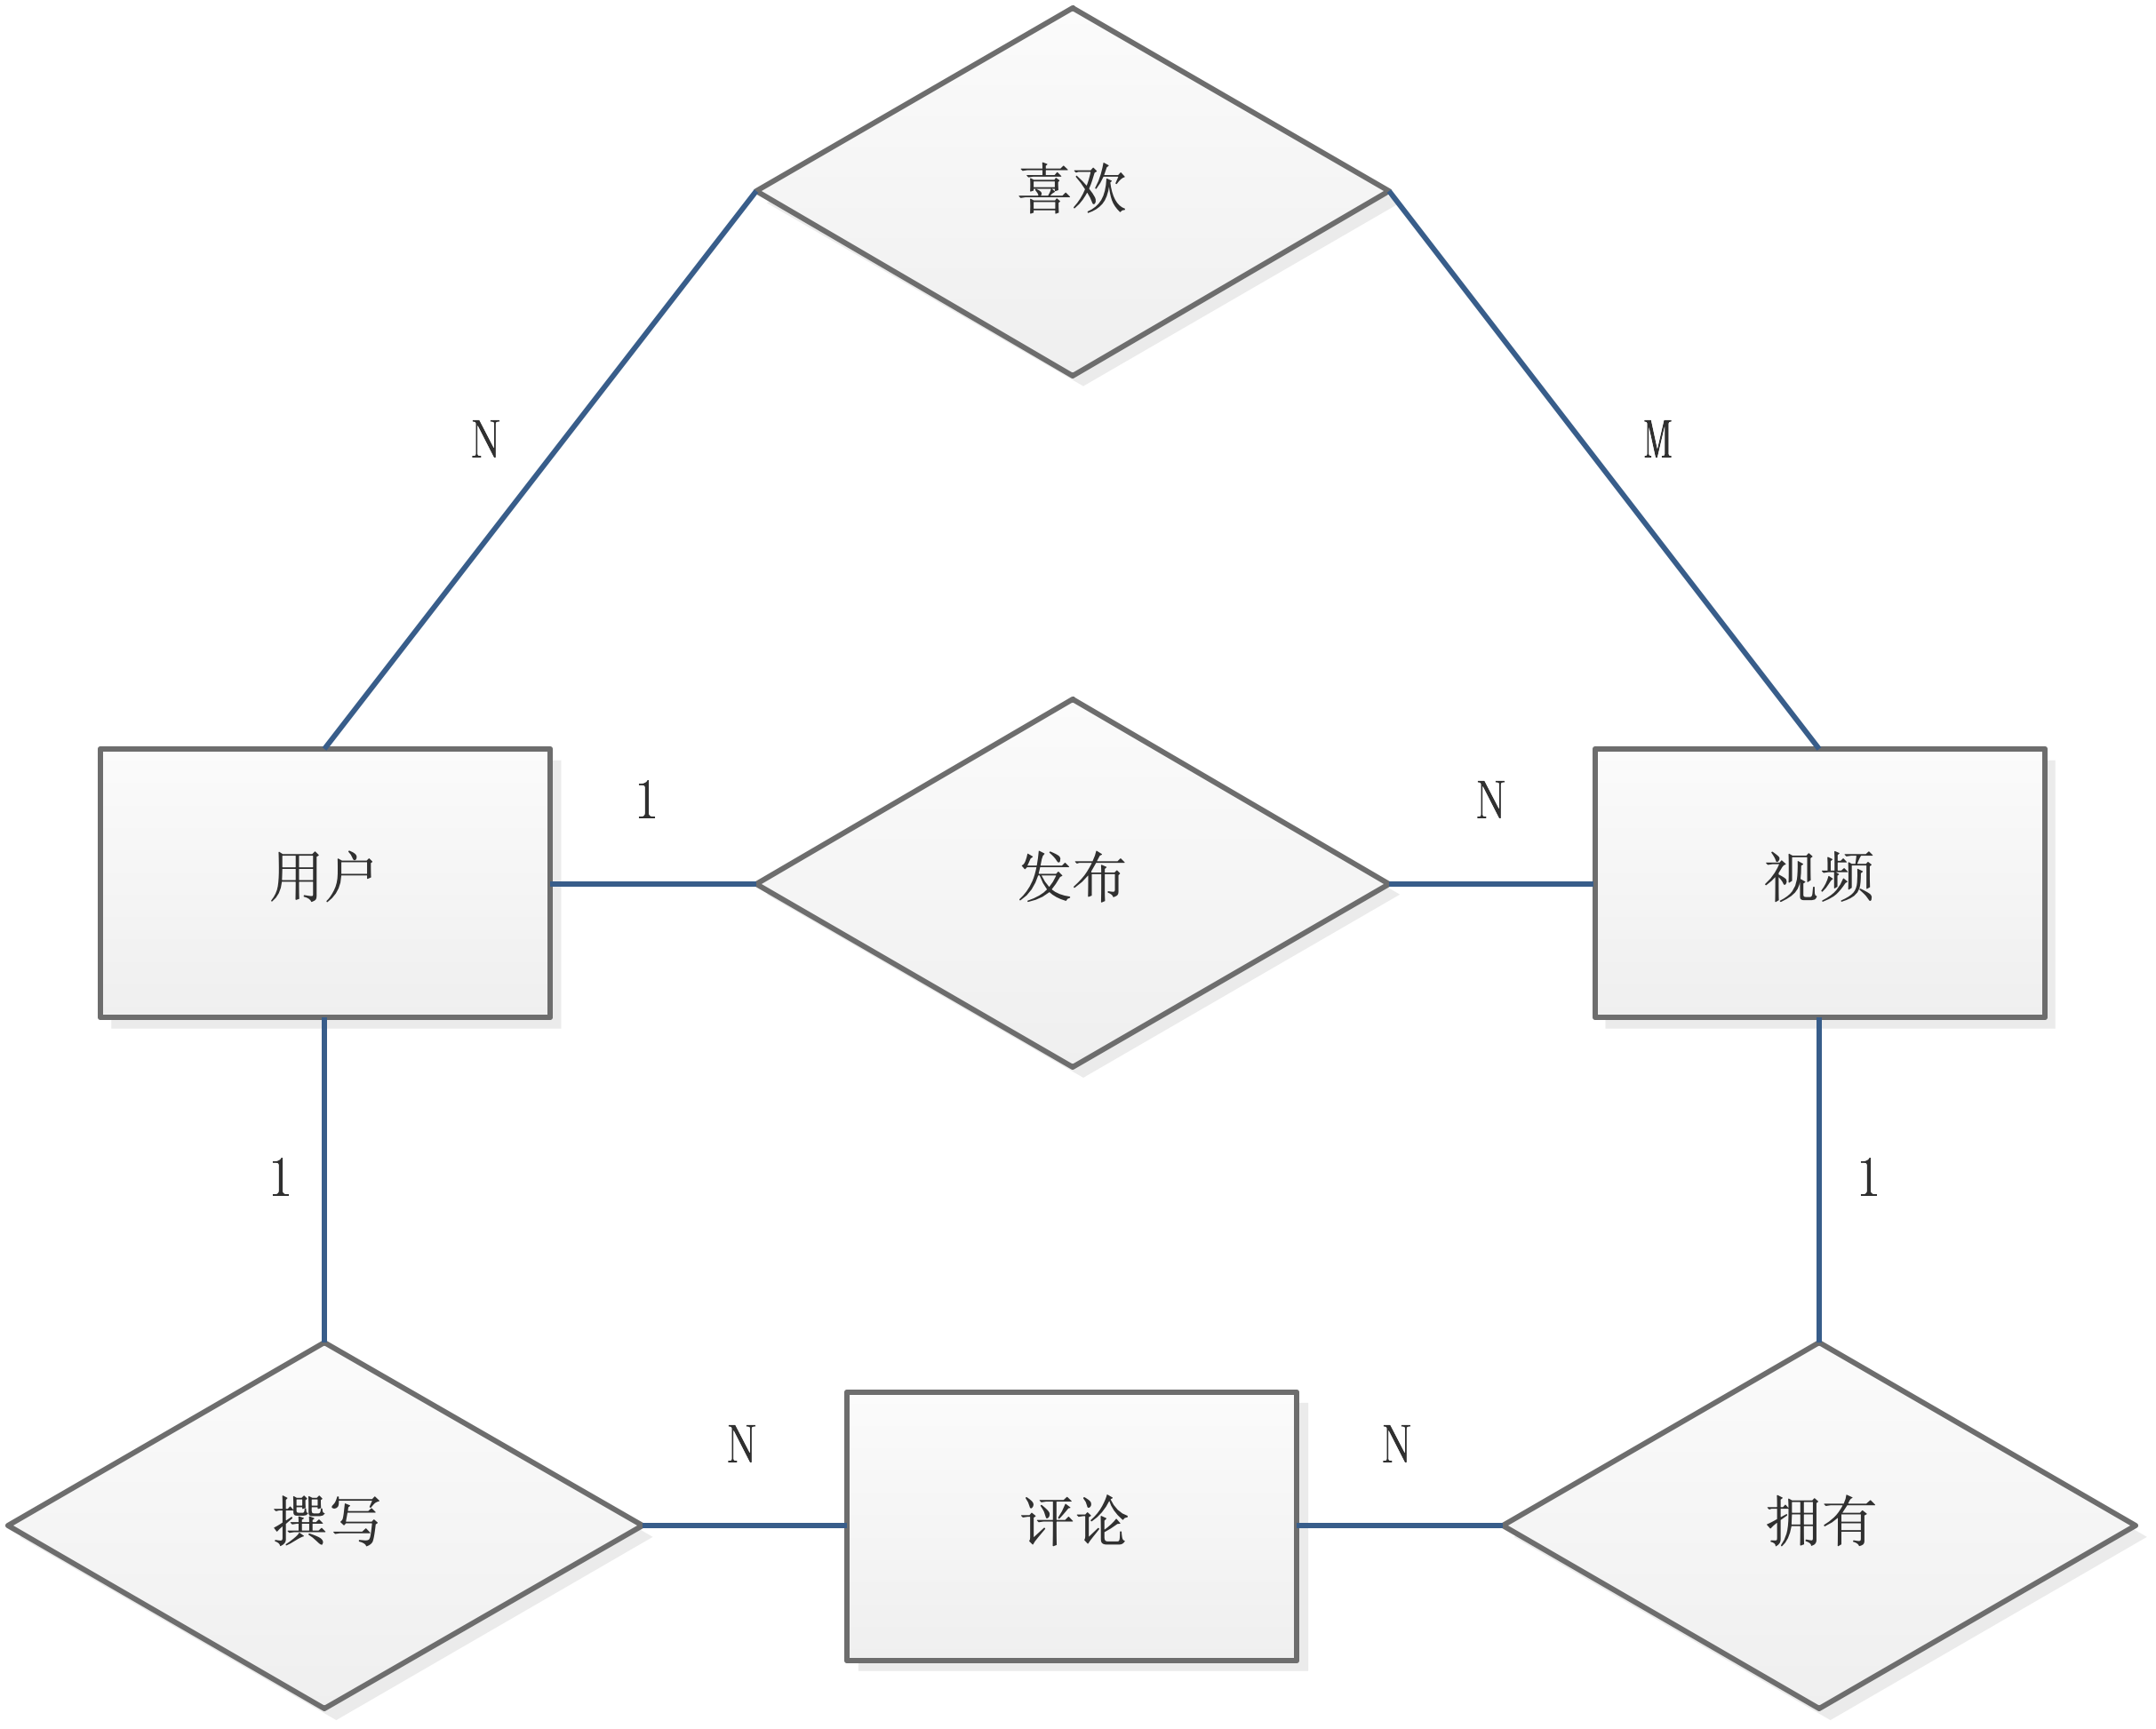
\includegraphics[width=0.6\textwidth]{dbs2.png}
    \caption{规范化后数据库 E-R 图}
    \label{fig:ER2}
\end{figure}

经过关系分解后,用户表与视频表中即不存在关于主属性的传递函数依赖,也不存在非主属性决定子,所以分解后整个关系达到了 BCNF,解决了之前可能出现的问题。

\subsection{数据库逻辑结构设计}

完成数据库的概念结构 (E-R 模型) 后开始设计数据库逻辑结构。这里我采用将 E-R 模型转换为关系模型的方法设计数据库逻辑结构。首先以 E-R 模型中各个实体为基础创建关系模式,然后创建实体间的联系。用户与视频间的发布联系是一个一对多联系,将其与 n 端对应的模式即视频关系模式合并。用户与视频间的关系为多对多关系,需单独设置一个关系模式储存。用户与评论以及视频与评论间的联系是一个多元联系,需单独设置一个关系模式储存。

本系统使用的关系模式为:用户模式(\uline{用户编号},用户名,用户密码,用户头像,用户统计信息)、视频模式(\uline{视频编号},视频名称,视频位置,视频作者,视频统计信息)、用户与视频间关系模式(\uline{用户编号},\uline{视频编号},关系类型)、用户、视频与评论关系(\uline{评论编号},用户编号,视频编号,评论类型,评论内容)。

\subsection{数据库物理结构设计与实施}

数据库物理结构由 MySQL 数据库管理系统默认生成,将上述关系模式转换为对应的结构化查询语句,并在 MySQL 中创建出相应的数据库表。完成数据库的实施之后,数据库设计完成。



\section{系统代码编写}

\subsection{系统整体设计}
本系统采用层次化结构进行开发,即将系统的功能由底至顶划分为若干层次,各层之间只能逐层单向调用,只能高级层次模块调用低级层次模块,系统各层次之间只提供相应接口,同时将具体实现屏蔽,这样增大了系统各模块内部的内聚度,减小了模块之间的耦合度,有利于系统开发。

\begin{figure}[!ht]
    \centering
    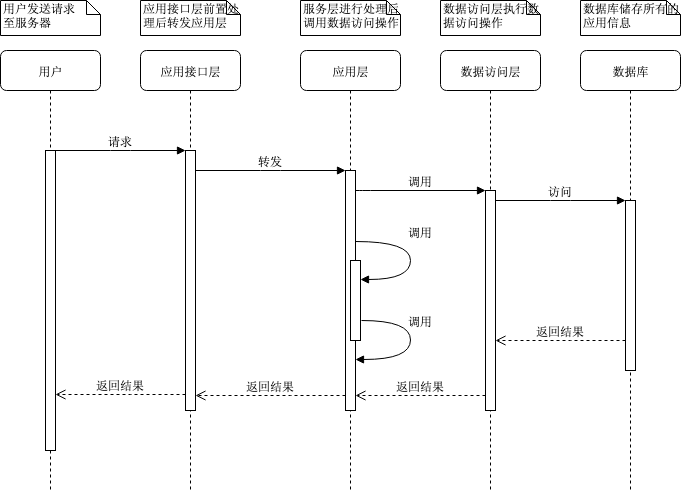
\includegraphics[width=0.6\textwidth]{soft1.png}
    \caption{短视频系统数据流图}
    \label{figs:soft1}
\end{figure}

根据短视频系统的功能要求,本系统被划分为公用功能层、数据访问层、服务层以及应用接口层。如图 \ref{fig:soft1} 所示,公用功能层是整个系统的最底层,含有许多供上层模块使用的静态依赖。数据访问层包含两部分一部分是数据访问对象模块,负责操作数据库;另一部分是实体对象模块负责保存数据库返回的结构。服务层依赖于数据访问层,它负责接收应用接口层发送的请求,做与数据相关的前期处理,封装相应的数据访问操作,并将结果进行处理后返回应用接口层。应用接口层接收用户请求,并作出权限判断等于前端有关的处理后将请求转发给服务层,接收结果后封装成响应结构返回给用户。

\subsection{系统具体实现}
本系统的应用接口层由 SpringMVC 实现、服务层由 Spring IoC 与 Spring AOP 实现、数据访问层基于 MyBatis 框架与 Spring AOP。

应用接口层包含了系统内所有的应用编程接口 (Application Programming Interface, API)。这些 API 主要可以分为三组:与用户相关的 API、与视频管理相关的 API以及处理用户与视频关系的 API。这些 API 均基于 SpringMVC 的注解式 API 声明。服务层包含了系统最主要的功能实现,主要使用 Spring IoC 提供的依赖注入功能获取数据访问依赖。数据访问层基于 MyBatis 框架,编写相应的实体类和访问接口后即可有 MyBatis 负责相应数据的读取与封装,并且使用 Spring AOP 实现对数据库事务的支持。



\section{短视频压缩编码初步实现实现}

短视频的压制与背景音乐合成由 FFmpeg 实现。FFmpeg 是一组音视频处理工具的集合。根据短视频应用的特性,我初步地将视频分辨率设为 1920 $\times$ 1080,帧率设置为 30 帧,码率采用 2 Mbps,编码采用 h.264 编码,封装格式采用 Mpeg4,兼容性较好,该压制属性可以保证视频中等清晰。

%\begin{lstlisting}
%ffmpeg -i input.MOV -vcodec h264 -profile:v high -level 5.1 -s 1920x1080 -preset slow -b:v 4M -maxrate 8M -bufsize 4M -r 29.97 output.mp4
%\end{lstlisting}



\section{数据库性能优化}



\section{视频编码优化}
